
Figures~\ref{fig:transformationsA}, \ref{fig:transformationsB} and \ref{fig:transformationsC} show the transformation rules from the elements of a $\pi$-SCM meta-model into elements of the $\pi$-{\sc Pews} meta-model. 
There are two groups of rules: those that transform service composition elements of the $\pi$-SCM to $\pi$-{\sc Pews} meta-models elements; and those that transform rules grouped by policies into {\em A-policy} types.
\begin{figure}
\centering{
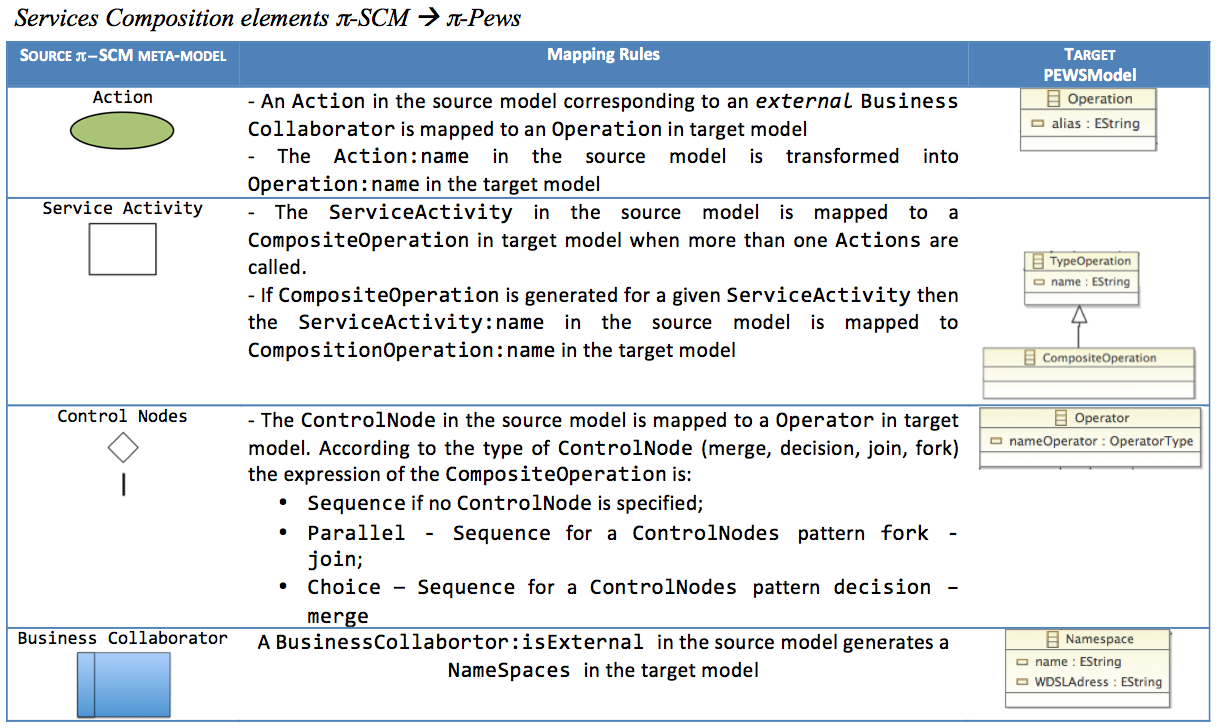
\includegraphics[width=0.96\textwidth]{figs/Mapping-1a.png}
}
\caption{ $\pi$-SCM to $\pi$-{\sc Pews} transformations (Services).}
\label{fig:transformationsA}
\end{figure}


\subsection{Transformation of $\pi$-SCM service composition elements into $\pi$-{\sc Pews} elements}

The transformation rules concerning service composition elements of $\pi$-SCM are shown in figure~\ref{fig:transformationsA}.
Named actions of $\pi$-SCM (represented by {\sc\em Action} and {\sc\em Action:name}) are transformed into a named class {\sc Operation} with a corresponding attribute name {\sc Operation:name}. 
Named service activities represented by the elements {\sc\em ServiceActivity}  and  {\sc\em ServiceActivity:name} of the $\pi$-SCM are transformed into named operations of the $\pi$-{\sc Pews} model, represented by the elements {\sc CompositeOperation} and {\sc CompositeOperation:name}. 
Workflow definitions are translated to the usual control flow structures, using the sequential, parallel and choice combinators of PEWS.

\begin{example}
In the scenario ``To Publish Music'' of Example~\ref{ex:toPublicMusic}, the service activity {\sf PublishMusic} of the $\pi$-SC model calls to two {\sf Activities} of type {\em UpdateMusic}, respectively concerning the {\em Facebook} and {\em Twitter} business services. 
The {\sf Composite Operation} named {\em PublishSong} of the $\pi$-{\sc Pews} model is obtained.
This operation uses the parallel constructor and it is written: {\sf PublishFacebook} $\parallel$ {\sf PublishTwitter}.
\end{example}



\subsection{Transformation of A-policies and rules into $\pi$-{\sc Pews}}

The {\em A-policies} defined for the elements of $\pi$-SCM are transformed into $\pi$-{\sc Pews} {\sc A-Policy} classes.
These classes keep their names, as expressed in the source model. 
The transformation of \textit{rules} is guided by the event types associated to these rules.
The $\pi$-SCM {\em A-policy} variables, given as {\sc\em $<$Variable:name, Variable:type$>$} are transformed into elements of type {\sc Variable} with attributes {\sc name} and {\sc type} of the $\pi$-SCM model.

As shown in Figures~\ref{fig:transformationsB} and~\ref{fig:transformationsC}, for an event of type {\sc\em Pre} the corresponding transformed rule is of type {\sc Precondition}; for an event of type {\sc\em Post} the corresponding transformed rule is of type {\sc Postcondition}; finally, for an event of type {\sc\em TimeRestriction} the corresponding transformed rule is of type {\sc Time}. 
The condition inside a $\pi$-SCM rule ({\sc\em Rule:condition}) is transformed into a class {\sc\em Condition:expression} where the attributes of the expression are transformed into elements of type {\sc Attribute}.

\begin{figure}
\centering{
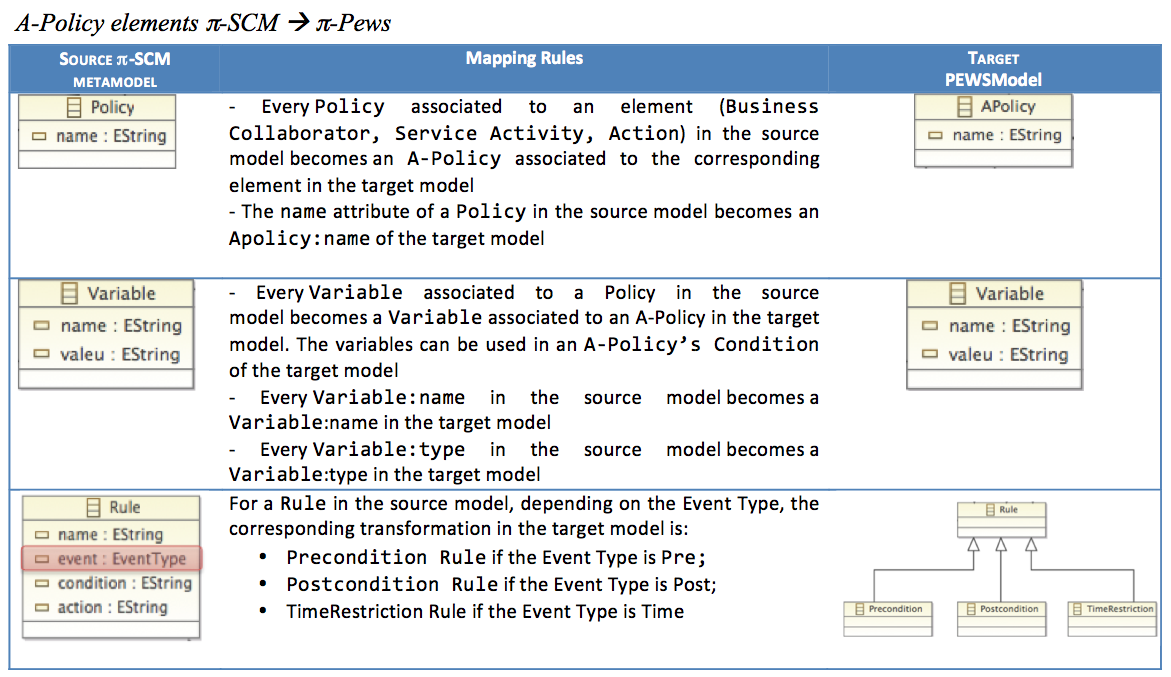
\includegraphics[width=0.96\textwidth]{figs/Mapping-1b.png}
}
\caption{ $\pi$-SCM to $\pi$-{\sc Pews} transformations (\textit{A-Policies}).}
\label{fig:transformationsB}
\end{figure}

\begin{example}
In the ``To Publish Music'' scenario of Example~\ref{ex:toPublicMusic}, the {\sf Policies} {\em OAuthPolicy} and {\em HTTPAuthPolicy} of the $\pi$-SCM model are transformed into {\em A-policies} of type {\sf Precondition} of the $\pi$-{\sc Pews} model. 
In both cases the events are of type {\sf ActivityPrepared}. 
These policies, as stated in the $\pi$-SCM model, are associated to {\sf Activities}. 
Their transformed counterparts are associated to operations {\em PublishFacebook} and {\em PublishTwitter}.
\end{example}

\begin{figure}
\centering{
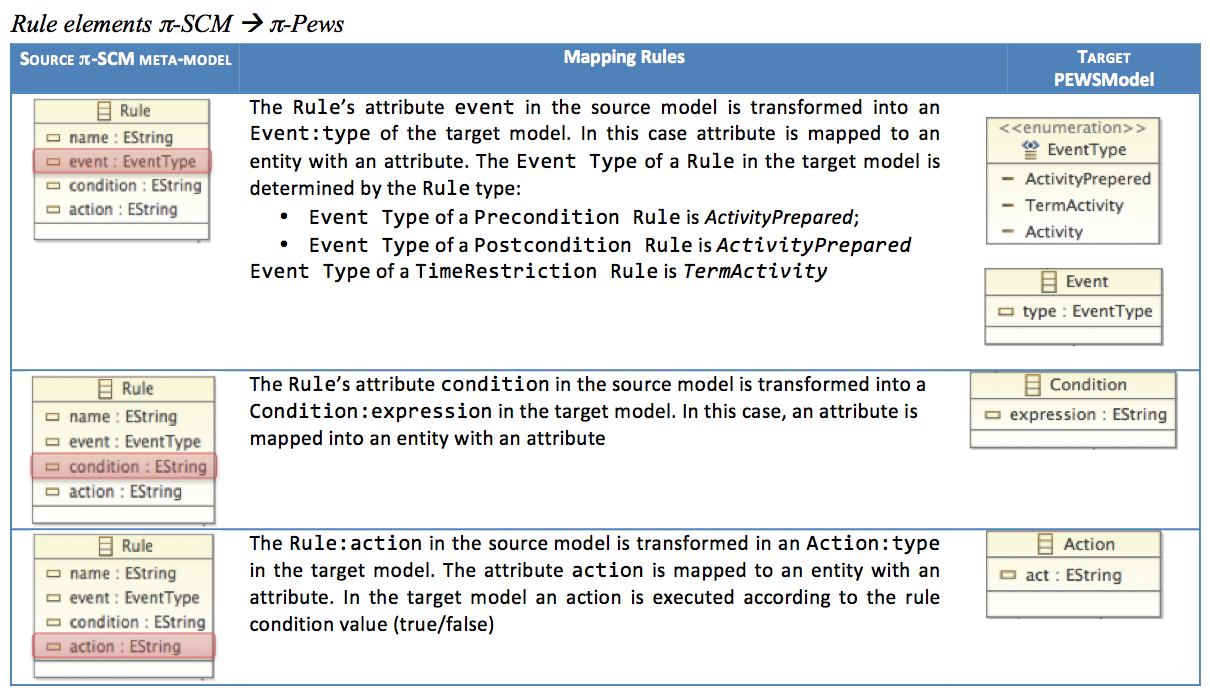
\includegraphics[width=0.96\textwidth]{figs/Mapping-1c.png}
}
\caption{ $\pi$-SCM to $\pi$-{\sc Pews} transformations (Rules).}
\label{fig:transformationsC}
\end{figure}
